
%Automata are more flexible than sequence-based approaches because they
%allow the hybrid control system to react to changes in the environment
%encountered during run time.  
{\large not talking about sequence approachs in this paper, but ideas
  this paragraph might be useful in intro} Like sequence-based
approaches, automata-based switching strategies are capable of
addressing multiple tasks; however, automata have the added advantage
of changing behaviors during runtime based on gathered information
without requiring re-planning.  Combining the policy composition
approach advocated in this thesis with automaton synthesis tools such
as those of~\cite{hadas_07} enables a constructive approach to
building a hybrid control policy whose continuous execution satisfies
high level specifications, while enabling the constrained system to
react to environmental changes.

{\large move idea here into the approach section }
This section presents several experiments and simulations using the synthesis
approach given in~\cite{hadas_07}.  As discussed in \resec{fully}, \cite{hadas_07}
uses a disjoint workspace decomposition and adjacency graph to choose policies based
on our fully actuated policies for idealized systems.  In contrast, this section
defines the specifications and automata synthesis in terms of the prepares graph.
This approach is more flexible because it can be applied to constrained systems, and
allows for overlapping policy domains.


The first example is termed the ``timid night watchman.''  The LAGR robot is tasked
with patrolling office corridors by visiting four checkpoints in turn.  If an
intruder is detected, as indicated by a binary sensor called `Intruder', the robot is
to ``run and hide'' in the small nook near the workspace center; after the intruder
is gone, the robot should resume patrolling.  The system also includes a `Hazard'
input; upon sensing a hazard, the robot should stop in place.  The robot resumes
motion when the hazard is clear.  The robot has three outputs: `Stop', which
indicates that the robot should cease executing its local policy and stop in place,
`CheckPoint', which means the robot is at a designated checkpoint, and $\CP_i$, which
encodes which policy is associated with the automaton node\footnote{Technically, this
  policy ID is encoded as a collection of binary outputs that encode the numeric
  identifier.  For clarity, we will use a simple binary proposition based on the
  numeric identifier for each policy.}.  $\CP_i$ is a binary proposition that is true
when the current state is in the domain of policy $i$.

The behavior is encoded in linear temporal logic (LTL) and input to the automaton
synthesis algorithm as $\varphi=\prl{\varphi_e \Rightarrow \varphi_s}$.  The LTL
formula $\varphi_e$ is an assumption about the inputs, and thus about the behavior of
the environment; the $\varphi_s$ formula represents the desired behavior of the
system.  More specifically,
\[
\bba{ccl}
\varphi_e & = & \varphi_i^e \wedge \varphi_t^e \wedge \varphi_g^e\,, \nonumber\\
\varphi_s & = &\varphi_i^s \wedge \varphi_t^s \wedge \varphi_g^s\,.\nonumber
\eba
\]
The formulas $\varphi_i^e$ and $\varphi_i^s$ describe the initial condition of the
environment and the system. $\varphi_t^e$ represents the assumptions on the
environment by constraining the next possible input values based on the current input
and output values. $\varphi_t^s$ constrains the transitions the system can make,
including obeying the prepares graph.  $\varphi_g^e$ and $\varphi_g^s$ represent the
assumed goals of the environment and the desired goals of the system, respectively.
% For a detailed description of these formulas the reader is referred to \cite{icra_07}.

The automaton synthesis algorithm used by~\cite{hadas_07} takes the initial
conditions, transition relations, and goals, then checks whether the specification is
realizable.  If it is, the algorithm extracts a possible, but not necessarily unique,
automaton that implements a strategy that the system should follow in order to
satisfy the desired behavior.  The automaton synthesis is viewed as a game played
between the environment, which controls the inputs, and the robot which controls the
outputs.  The two players have initial conditions defined by $\varphi_i^e$ and
$\varphi_i^s$.  The way the game is played is that at each step, first the
environment makes a transition according to $\varphi_t^e$, and then the system makes
its own transition according to $\varphi_t^s$.  If the environment can falsify
$\sigma = \prl{\varphi_g^e\Rightarrow\varphi_g^s}$ regardless of the system
transition, we say that the environment is winning and the desired behavior is
unrealizable; this means that there is no automaton that can satisfy the
requirements.  However, if the system can satisfy the desired behavior encoded by
$\sigma$, no matter what the environment does, we say that the system is winning and
we can extract an automaton.

Note that there are two ``ways'' for the system to win. It wins if
either $\varphi_g^s$ is satisfied, i.e.  the system reaches its goals,
\textbf{or} $\varphi_g^e$ is falsified.  The later case implies that
if the environment does not satisfy its goals (either a faulty
environment or the system interfered), then a correct behavior of the
system is no longer guaranteed.  Furthermore, if during an execution
of the automaton the environment violates its own transition relation
encoded by $\varphi_t^s$, the automaton is no longer valid.  The
implication of this is discussed below.

Using the specific ``timid night watchman'' task, the behaviors are encoded as
follows.  The environmental inputs are `Hazard' and `Intruder'.  The system outputs
are those that specify which policy to activate, the `Stop' command, and the
`CheckPoint' flag.  The Hazard input is initially clear, so $\varphi_i^e =
\NOT\mrm{Hazard}$.  There are no other assumptions about the environment;
therefore,$\varphi_t^e = \ALWAYS\TRUE$ and $\varphi_g^s = \ALWAYS\EVENTUALLY\TRUE$.
That is `Intruder' input can have any initial value, and the inputs can change at
will, with no final goal.  The system state is assumed to be in one of two initial
policy domains, the initial policies are not checkpoints, and the system is not
stopped by hazard; therefore,
\[\varphi_i^s = \prl{\CP_1
  \OR\CP_3}\,\AND\,\NOT\STOP\,\AND\,\NOT\mrm{CheckPoint}\,.\] 
The system transitions include knowledge of the prepares graph; thus, using the same
prepares graph as \resec{lagr_total_order}, define
\[\varphi_\Gamma^s = \bigwedge_i \;\Box(\Phi_i\;\Rightarrow\;\prl{\bigcirc
  \Phi_i\bigvee_{j\in \mrm{SuccessorsOfPolicy}_i}\bigcirc \Phi_j}\,.
\] In English, ``it is always true that if the current state is in $\Do{\Phi_i}$ this
time step, the next step will find the state in either $\Do{\CP_i}$ or one of its
successors.''  The set of successors is defined by the prepares graph.  The system
stops if and only if there is a hazard sensed; that is $\varphi_\mrm{haz}^s =
\prl{\NEXT\mrm{Hazard}\IFF\NEXT\STOP}$~\footnote{The ``if and only if'', denoted
  $\IFF$, is a binary proposition that is true if both sides have the same truth
  value, and false otherwise.  Thus, $\prl{\FALSE\IFF\FALSE}$ is true.}.  The system
also encodes that the policy reference does not change if the system stops; that is,
\[\varphi_\mrm{stop}^s = \ALWAYS\prl{\prl{\NEXT\mrm{Hazard}
    \OR\STOP}\,\AND\,\CP_i} \Rightarrow \NEXT\CP_i\,.\] If an intruder is
sensed, and the system is hidden in the nook, the system should stay in the nook;
that is
\[\varphi_\mrm{hide}^s =
\ALWAYS\prl{\NEXT\mrm{Intruder}\,\AND\,\CP_1}\Rightarrow\NEXT\CP_1\,,\]
where $\CP_1$ is the policy that stops the system in the nook.  The system should
resume patrol if the intruder is not sensed; that is
\[\varphi_\mrm{unhide}^s =
\ALWAYS\prl{\NOT\NEXT\mrm{Intruder}\,\AND\,\NOT\mrm{Hazard}\,\AND\,\NOT\STOP}\Rightarrow\NOT\NEXT\CP_1\,.\]
If the robot is at a checkpoint, the CheckPoint output is set; that is
\[\varphi_\mrm{chk}^s=\ALWAYS\prl{\prl{\NEXT\CP_{70}}\,\OR\, \prl{\NEXT\CP_{258}}\,\OR\, \prl{\NEXT\CP_{200}}\,\OR\,
  \prl{\NEXT\CP_{291}}\,\IFF\,\NEXT\mrm{CheckPoint}}\,,\] where 70, 258, 200, and 291
denote the policy domains assigned as checkpoints.  Together, the system transitions
are encoded as
\[\varphi_t^s = \varphi_\Gamma^s\,\AND\,\varphi_\mrm{haz}^s\,\AND\,
\varphi_\mrm{stop}^s\,\AND\,\varphi_\mrm{hide}^s\,\AND\,\varphi_\mrm{unhide}^s\,\AND\,\varphi_\mrm{chk}^s\,.\]
The desired behavior, given as the system goal, is
\[\varphi_g^s=\left\{
\bba{c}
\ALWAYS\EVENTUALLY\prl{\CP_{70}\,\OR\,\mrm{Intruder}\,\OR\,\STOP}\,\AND\\
\ALWAYS\EVENTUALLY\prl{\CP_{258}\,\OR\,\mrm{Intruder}\,\OR\,\STOP}\,\AND\\
\ALWAYS\EVENTUALLY\prl{\CP_{200}\,\OR\,\mrm{Intruder}\,\OR\,\STOP}\,\AND\\
\ALWAYS\EVENTUALLY\prl{\CP_{291}\,\OR\,\mrm{Intruder}\,\OR\,\STOP}\,\AND\\
\ALWAYS\EVENTUALLY\prl{\CP_1\,\OR\,\NOT\mrm{Intruder}\,\OR\,\STOP}
\eba
\right.
\,.
\]
The automaton synthesis satisfies the goals in order.  Therefore, as long as the
intruder is not seen, the automaton implicitly encodes go from 70, to 258, to 200,
and finally to 291 before repeating the cycle. 
 
\begin{figure}[bt]
  \centering 
   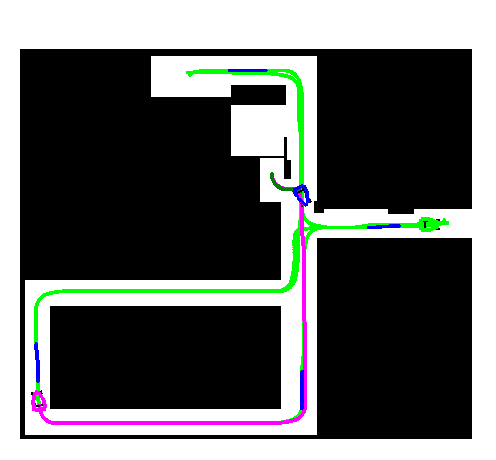
\includegraphics[width=3in]{graphics/AutRnd5_Sim8_path.eps}

   \caption[`LAGR' timid night watchman.]{A simulation of path induced by an
     automaton that encodes the behavior patrol the corridors by visiting four
     specific policy domains is shown.  Upon sensing a `Intruder', the ``timid night
     watchman'' goes and hides in the corner until the intruder leaves.  Three robots
     are shown: the initial pose to the right, the final pose when execution is
     terminated near the middle, and the pose at which the intruder is detected in
     the lower right.  }
   \label{fig:lagr_Aautomaton_full_path}
\end{figure}

Together, the automaton and policy suite serve as a hybrid control policy.  For these
specifications, the extracted automaton has 2400 nodes.  Executing the local control
policies as specified by the automaton induces a continuous system evolution that
satisfies the high level specification.  At the start of execution, we search the
entire automaton as a list of nodes until a node is found that has the correct input
state (Intruder = false) and whose associated policy contains the initial pose.  This
approach, which allows starting from some arbitrary initial pose, works for this
particular scenario because of the cyclic behavior of the scenario; other scenarios
might require that the robot start in the domain of a policy in an explicit set of
initial policies.  A simulation run is shown in \refig{lagr_Aautomaton_full_path}.
The intruder detector is triggered at an arbitrarily specified time.

The automaton governs the selection of local control policies.  The automaton
transitions between nodes as the system pose enters the domain of a policy associated
with a child node of the current automaton node.  In other words, from node $p_i$, at
each time step\footnote{The policies are designed as continuous control laws;
  however, the implementation on a computer induces a discrete time step.  We assume
  the time step is short compared to the time constant of the closed-loop dynamics.},
the values of the binary sensor inputs are evaluated. Based on these inputs, all
valid successor nodes are determined. If the vehicle is in the domain of policy
$\Phi_{l}$, which is associated with a valid automaton successor node $p_j$, the
transition is made.  Otherwise, if the vehicle is still in the domain of $\Phi_{k}$,
which is the active policy associated with node $p_i$, the execution remains in node
$p_i$.  If a node has more than one child node that represents a valid transition,
the choice can be made arbitrarily.  For these experiments, the first valid
transition as defined by the synthesis algorithm is chosen.  This execution based on
continuous motion is equivalent to the discrete execution of the automaton
\cite{fainekos_05a,belta_06}.


\begin{figure}[bt]
  \centering 
  \psfrag{2500}{2500}
  \psfrag{2000}{2000}
  \psfrag{1500}{1500}
  \psfrag{1000}{1000}
  \psfrag{500}{500}
  \psfrag{Time (s)}{Time (s)}
  \psfrag{Node ID}{Node ID}
  \psfrag{Automaton Nodes}{}

    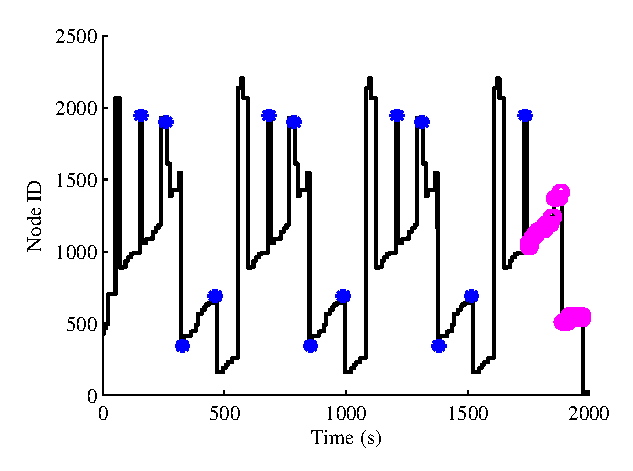
\includegraphics[width=3in]{graphics/AutRnd5_Sim8_nodes.eps}

    \caption[`LAGR' timid night watch automaton node switching.]{As the system
      executes, the automaton changes nodes based on the discrete inputs and
      inclusion of the current pose in a given policy domain.  The graph shows three
      distinct phases.  The thirteen points marked with '*' indicated the check
      points passed.  The thickest portion, which is actually closely spaced
      `$\circ$' symbols, shows the portion where the intruder is detected.  Notice
      that the system makes multiple passes past each checkpoint before the intruder
      is detected.}
   \label{fig:lagr_Aautomaton_full_nodes}
\end{figure}


\refig{lagr_Aautomaton_full_nodes} shows the progression of the system through the
automaton nodes as the system moves through the environment.  Note the cyclic nature
as the system completes three patrols before the intruder is detected.  As the
automaton state transitions, so does the associated policy as shown in
\refig{lagr_Aautomaton_full_policies}.

\begin{figure}[bt]
  \centering 
  \psfrag{3500}{3500}
  \psfrag{3000}{3000}
  \psfrag{2500}{2500}
  \psfrag{2000}{2000}
  \psfrag{1500}{1500}
  \psfrag{1000}{1000}
  \psfrag{500}{500}
  \psfrag{Time (s)}{Time (s)}
  \psfrag{Policy ID}{Policy ID}
  \psfrag{Policy}{}
   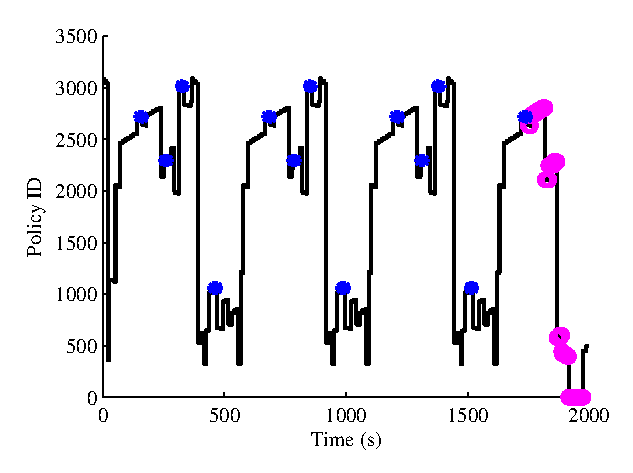
\includegraphics[width=3in]{graphics/AutRnd5_Sim8_policies.eps}

   \caption[`LAGR' timid night watch policy switching.]{Each node in
     the automaton is associated with a particular policy in the
     suite.  As the system executes, the local policies are activated
     by the automaton based on the local pose estimate.The graph shows
     the same three distinct phases as
     \refig{lagr_Aautomaton_full_nodes}.}
   \label{fig:lagr_Aautomaton_full_policies}
\end{figure}

In this execution strategy, the continuous evolution of the system governs the
discrete transitions in the automaton; therefore, the resultant transitions are
asynchronous, and not governed by a fixed time step.  In this current implementation,
the discrete inputs act as guards on the automaton transitions; the discrete input
must match the value associated with the child node to allow transition into the
child node, but does not force transition out of the current node.  Another approach
could check the discrete input at each update step and force transitions out of a
given automaton node if the inputs do not match the reference input.  This would
require that each node has a child with the same policy reference, but different
discrete inputs .

%\FloatBarrier

\begin{figure}[bt]
  \centering 
   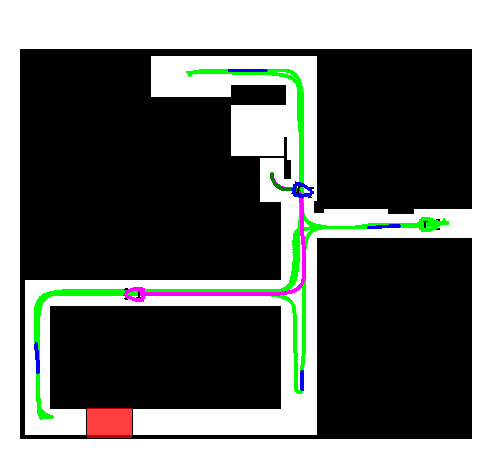
\includegraphics[width=3in]{graphics/AutRnd5_Sim7_path.eps}

   \caption[`LAGR' timid night watch re-planning.]{As new information
     becomes available, such the obstacle in the lower corridor, the
     automaton synthesis formulates a different automaton based on
     changes to the prepares graph.  The new automaton preserves the
     correct behavior.}
   \label{fig:lagr_Aautomaton_blocked}
\end{figure}


If the prepares graph changes, the automaton synthesis algorithm must be re-run.
\refig{lagr_Aautomaton_blocked} shows the simulated path taken when an automaton is
synthesized for the prepares graph with 24 policies associated with the lower
corridor invalidated.  The resultant automaton contains 2580 nodes; its execution
correctly satisfies the original specification by only invoking valid policies.

%\FloatBarrier

The automaton synthesis approach guarantees the correct behavior under very
reasonable assumptions.  First, the automata synthesis only returns an automaton if
the specification is realizable for the given policy suite and associated prepares
graph. Second, given a realizable specification, the algorithm is guaranteed to
produce an automaton such that all its executions satisfy the desired behavior {\bf
  if} the environment behaves as assumed.  The construction of the automaton is done
using LTL statements that encode admissible environment behaviors; if the environment
violates these assumptions, the automaton is no longer correct.  Since the
specifications encode the transitions allowed by the prepares relationship, the only
case in which the system pose is not in the domain of $\Phi_{k}$, or in any successor
$\Phi_{l}$, is if the environment behaved ``badly.''  That is, either some
disturbance caused the policies to violate the prepares relationship, or the
environment violated assumptions governing the allowable discrete inputs.  This later
case requires careful sensor design, with only those restrictions that are
necessary.  Either case invalidates the automaton.  In the event that a valid
transition does not exist, the automaton executive raises an error flag, and halts
the system.  A new plan must be requested.

Unfortunately, for real systems disturbances are a fact of life.  Policies may be
designed to be as robust as possible, but disturbances may still take the system out
of the domain of a currently executing policy.  Often these disturbances are simply
due to pose estimation updates as described above.  The hybrid control system should
have a method of recovery, which will likely require some knowledge of the hybrid
control system and task.  For the task described in this section, our approach is to
search the automaton as a list of nodes until a node whose associated policy contains
the current pose estimate and whose discrete input matches the current sensor value;
as is done for the initial condition. This works in this example because of the
cyclic nature of the task.  

A more fundamental problem is when the disturbance takes the system
outside the domain of all policies in the automaton.  Depending on the
initial specification, the automaton synthesis does not necessarily
use every available policy.  As with sequence-based approaches, this
has a negative impact on the overall robustness of the policy
composition technique relative to the collection of available
policies.  This thesis considers two approaches to addressing the
problem of unused policies.

The first approach explicitly allows the initial condition to be in any available
policy and have any allowable sensor value.  The assumption during synthesis that the
system is in one of two initial policy domains is made to limit the size of the
automaton.  No assumptions about the initial policies could be made such that
$\varphi_i^s=\NOT\STOP$; this would force the automaton to include all policies, but
would greatly increase the size of the synthesized automaton.  The particular
implementation of the synthesis algorithm used in this thesis precluded this
approach; this is not a theoretical issue, later work will build a more robust
synthesis tool to address this implementation issue~\cite{hadas_pc}.

The second approach, which is used in these experiments, is to augment the
synthesized automaton to add nodes for each unused policy/sensor combination.  If a
policy is unused by the original automaton, but prepares another policy that is used
for all input combinations, then a node is added to the automaton with the unused
policy as a reference.  This added node ignores the sensor inputs.  The children of
the added node are all nodes in the automaton whose associated policies are prepared
by the added node's policy or have the same policy reference.  Since all input
combinations are covered, a valid child transition will eventually exist.  This
process is repeated until all policies that prepare others are added to the
deployment.  This approach maximizes the overall hybrid control policy domain for the
given collection of domains, while adding the smallest number of nodes to the
automaton.  This gives the system a way to ``get back on track.''  If the disturbance
causes the system pose to exit the domains of every policy in the suite, then the
hybrid control policy will stop the robot and cease execution.  Only by adding
additional policies, and regenerating the automaton can the system recover.


\begin{figure}[bt]
  \centering 
   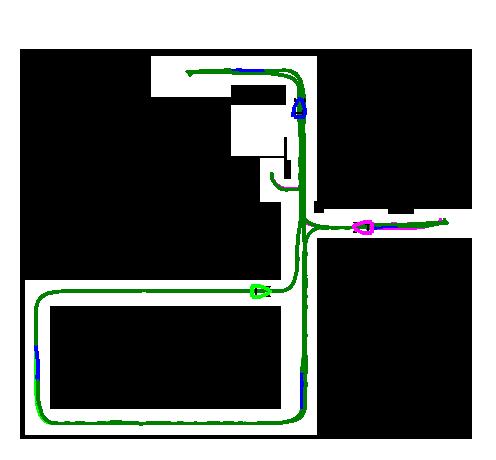
\includegraphics[width=3in]{graphics/AutRnd5_Run4_path.eps}

   \caption[`LAGR' timid night watch experiments.]{Actual run on
     LAGR robot.  Here, the robot resumes patrolling after hiding
     early in the experiment.}
   \label{fig:lagr_Aautomaton_experiments}
\end{figure}

\refig{lagr_Aautomaton_experiments} shows an example run using the augmented
automaton.  During the experimental runs, the intruder is signaled at will via a
switch on the remote control used an emergency stop.  The experiment successfully
satisfies the specification.  \refig{lagr_Aautomaton_experiments_nodes} shows the
progression of nodes during execution.  Note that the nodes above 2400 are augmented
nodes; without these, the execution would have ceased earlier due to disturbances.
Given the augmented automaton, the system is able to search for a node whose policy
contains the current pose.  Eventually, the execution did quit when a disturbance
finally took the system out of the domain of all the policies.
\refig{lagr_Aautomaton_experiments_policies} shows the policy switching induced by the
augmented automaton.  The experiment was repeated several times; the automaton
successfully induced the correct behavior each time until disturbances caused the
system to terminate; this points to the need for more policies to be added to the
policy suite.

\begin{figure}[bt]
  \centering 
  \psfrag{3500}{3500}
  \psfrag{3000}{3000}
  \psfrag{2500}{2500}
  \psfrag{2000}{2000}
  \psfrag{1500}{1500}
  \psfrag{1000}{1000}
  \psfrag{500}{500}
  \psfrag{Time (s)}{Time (s)}
  \psfrag{Node ID}{Node ID}
  \psfrag{Automaton Nodes}{}
   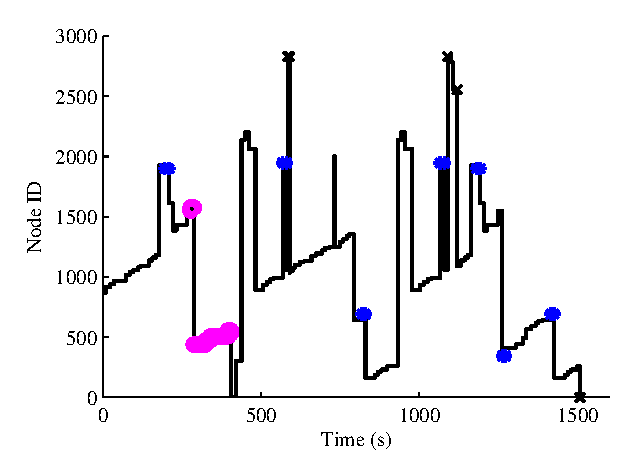
\includegraphics[width=3in]{graphics/AutRnd5_Run4_nodes.eps}

   \caption[`LAGR' node switching during experiment]{Node switching with
     invocations of augmented nodes shown by 'x'; the controller would have ceased
     execution were it not for these added nodes.}
   \label{fig:lagr_Aautomaton_experiments_nodes}
\end{figure}



\begin{figure}[bt]
  \centering 
  \psfrag{3500}{3500}
  \psfrag{3000}{3000}
  \psfrag{2500}{2500}
  \psfrag{2000}{2000}
  \psfrag{1500}{1500}
  \psfrag{1000}{1000}
  \psfrag{500}{500}
  \psfrag{Time (s)}{Time (s)}
  \psfrag{Policy ID}{Policy ID}
   \psfrag{Policy}{}
  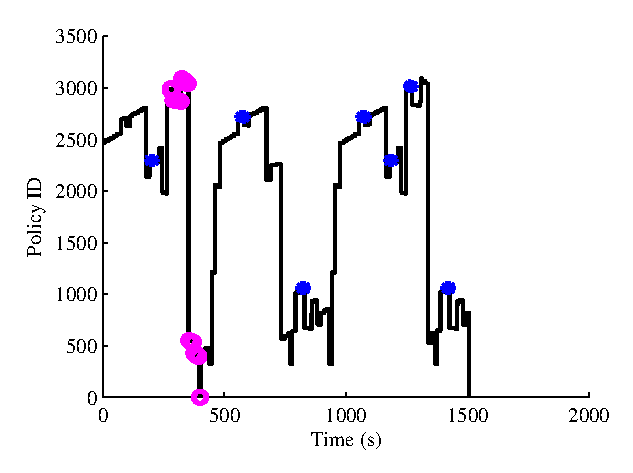
\includegraphics[width=3in]{graphics/AutRnd5_Run4_policies.eps}

   \caption[`LAGR' policy switching during experiment]{Policy switching during an experiment.}
   \label{fig:lagr_Aautomaton_experiments_policies}
\end{figure}

The drawback to the augment and search approach is that there is no history;
therefore, the system will sometimes repeat an earlier portion of the patrol loop,
prior to visiting the other nodes.  This problem could be addressed by adding an
output that encodes which ``downstream'' check point will be encountered next, and
using this information to guide the search for a valid node.  This requires
associating each policy with the closest checkpoint before the synthesis.  One
possible approach is to choose the checkpoint that generates the least cumulative
cost for a given policy from a set of costs generated by considering each checkpoint
as the goal of a total ordering.  During disturbance recovery, the system searches
for a node whose associated policy domain contains the current pose and whose
``ClosestCheckpoint'' output matches the assigned checkpoint for that policy.

%\FloatBarrier%afterpage{\clearpage}

The automata-base approach is capable of producing complex behaviors, which allow the
system to react to changes in the environment via the binary environmental inputs.
Additionally, the automata-based approach allows the system to exhibit desirable
limit cycles; in this example, repeatedly patrolling a hallway.  Thus automata-based
approaches are more suitable for repetitive tasks than order-based approaches.  That
said, the automata should make use of all available policies, and provide a method of
recovery, in order to maintain robustness to disturbance that is the hallmark of
order-based approaches.

% \subsection{Ackermann Steered Car-like Parking Simulations}
% \label{sec:automaton_ackermann_automaton}

% \begin{figure}[bt]%[ht]
% \begin{center}

%  \vspace{0.2in}

%  \includegraphics[width=4in]{graphics/sim_parking_demo.eps} 

%   \caption[Local parking behavior induced by meta-policy]{Parking behavior induced by
%     the composition of local policies.  The feedback control policies guarantee the
%     safety of the maneuver.}
% \label{fig:automata_parking}
% \end{center}
% \end{figure}

% This section provides an example of policy-based planning with the more complex
% system model of an Ackermann steered car.  Here, the scenario is one of searching for
% an available parking space, and then parking.  The environment is known; what is
% unknown is whether a given parking space is available or occupied.  The system has a
% local sensor for detecting open parking spaces; thus, the system must search for an
% available parking space by systematically driving past all the parking spaces.  If an
% open parking space is found, the system changes behavior from searching to parking,
% and executes the parking maneuver as illustrated in \refig{parking}.  The results
% demonstrate coupled planning and control for a complex system that exhibits complex
% behaviors that change based on reactions to the changing environment.

% \begin{figure}[bt]
%   \centering
%   \includegraphics[width=0.75\linewidth]{graphics/sim_parking_run_0_world.eps}
%   \caption[Environment for parking simulations]{The environment has 40 parking spaces
%     arranged around the middle city block.  Initially, there are five empty parking
%     spaces randomly chosen in the environment.}
%   \label{fig:automaton_acker_parking_world}
% \end{figure}

% The environment, shown in \refig{automaton_acker_parking_world}, consists of two city blocks
% accessible from ten entering roads.  Each road consists of two lanes that follow the
% American standard of driving on the right side.  One block is surrounded by 40
% parking spaces; 20 for the clockwise direction and 20 for the counterclockwise
% direction. The entry/exit points are labeled 1-10 clockwise starting from the
% north/south lanes at the top left of the environment.  The parking spaces are
% identified with a numeric identifier adjacent to each space.  The roadway lanes and
% parking spaces are sized for an urban environment.  The robot system uses an
% Ackermann steered kinematic model that controls the forward velocity and the rate of
% steering angle change; see \reapp{robots} for details.

% \begin{figure}[bt]
%  \begin{center}
%  \begin{minipage}[b]{\linewidth}
%  \begin{minipage}[b]{0.48\linewidth}
%   \centering 
%   \includegraphics[width=\linewidth]{graphics/parkway_details_parking.eps}

%  {\scriptsize a) Policies for parking.}
%    \end{minipage}
%  \hspace{0.03\linewidth} % To get a little bit of space between the figures
%  \begin{minipage}[b]{0.48\linewidth}
%    \centering 
%    \includegraphics[width=\linewidth]{graphics/parkway_details_leaving.eps}

%   {\scriptsize b) Policies for leaving}
%  \end{minipage}

%  \end{minipage}
 
%  \caption[Parking policy details]{Details of policies used for parking
%    and leaving.  The policies, which are shown relative to the cache
%    reference point, are shown wider than normal to show details.  Six
%    policies are associated with parking.  Five policies are used to
%    exit a parking space and prepare policy in the traffic lane.}
%   \label{fig:automata_parkway_details}
% \end{center}
% \end{figure}

% The parking demonstrations use a collection of 16 \PF style policies, which are
% instantiated in the policy cache relative to the origin.  The cache includes policies
% for traveling straight down a roadway lane, for parking and leaving a given space,
% and for turning at intersections.  \refig{parkway_details} shows examples of the
% policies for parking and leaving, which treated as meta-policies for planning
% purposes.  Associated with the inlet policy of the parking policy is a sensor that
% determines whether the parking space is available.  If the parking space is
% unavailable, then the parking meta-policy prepares some other policy further down the
% roadway lane.  \refig{parkway_intersection} shows an example intersection, the
% deployed policies, and the extent of the robot body into the workspace.  Since this
% is a simulation, only those policies needed for basic traffic are deployed.  No
% attempt is made to fill the free pose space in order to provide robustness.


% \begin{figure}[bt]
%  \begin{center}
%  \begin{minipage}[b]{\linewidth}
%  \begin{minipage}[b]{0.48\linewidth}
%   \centering 
%   \includegraphics[width=\linewidth]{graphics/parkway_intersection_lanes.eps}

%   \end{minipage}
%  \hspace{0.03\linewidth} % To get a little bit of space between the figures
%  \begin{minipage}[b]{0.48\linewidth}
%    \centering 
%    \includegraphics[width=\linewidth]{graphics/parkway_intersection_padded.eps}

%  \end{minipage}

%  \begin{minipage}[b]{0.48\linewidth}
%   \centering 

%   {\scriptsize a) Connected policy domains projected into workspace}

%  \end{minipage}
%  \hspace{0.03\linewidth} % To get a little bit of space between the figures
%  \begin{minipage}[b]{0.48\linewidth}
%    \centering 

%    {\scriptsize b) Body extent over the policy domains}

%  \end{minipage}
%  \end{minipage}
 
%  \caption[Policies deployed at intersection]{Deployment of policies at an
%    intersection.  The polices include those that pass straight through the
%    intersection, as well as left and right turns.  Other policies are used to tie the
%    straight sections to the turns.  The policy domains, which are widened to increase
%    visibility, appear as thick lines in (a).  }
%   \label{fig:automata_parkway_intersection}
% \end{center}
% \end{figure}

% For the simulations in this section, a total of 306 policies are deployed in the
% environment.  The regularity of the environment allows an automated approach to
% policy instantiation based on a collection of reference points defined relative to
% the intersections and parking spaces.  The policy total includes 40 parking
% meta-policies and 40 leaving meta-policies, as well as 24 each left, right and
% straight maneuvers at the six intersections.  Policies to enter and leave the
% environment are added at the 10 roadways connecting the environment to the outside
% world.  Given the suite of 306 policies, the prepares graph is automatically defined
% as described in \resec{nonholo}.

% In many ways, the policy suite and prepares graph can be viewed as information that
% the environment communicates to the vehicle.  One can envision a scenario where this
% information is passed to a vehicle as the system enters a new neighborhood.  The
% vehicle could quickly verify that its system model and input constraints are valid
% for the policies defined in the cache; multiple suites and caches could be defined
% for a range of vehicle sizes.  Given a valid suite of policies, the vehicle is then
% free to plan its local behavior over this environment.

% %\FloatBarrier%afterpage{\clearpage}

% \subsubsection{Basic Parking Scenarios}
% \label{sec:automaton_acker_parking}

% The basic scenario considers a single car that must park in the
% environment.  The environmental input is a sensor called `\PARK' that
% tells the car if a parking space is available; the system output
% identifies which policy to activate.  The car may enter from any of
% the ten roadways connecting to the two blocks; that is
% $\varphi_i^s=\OR_{i\in\mrm{InitialPolicies}} \CP_i$.  Since these are
% not adjacent to a parking space, $\varphi_i^e = \NOT\PARK$.  The car
% can only determine whether there is a free parking space if we are in
% a policy next to it. This means that `Park' cannot become true if the
% vehicle is not next to a parking space or in one. Also, for
% implementation reasons, we assume that the input `Park' remains true
% after parking.
% $$\varphi_t^e = \left\{\begin{array}{c}
%     \ALWAYS\prl{\;\;\brl{\;\;\;\;\prl{\NOT \prl{\bigvee_{i\in \mrm{ParkPolicies}}\Phi_i}}\;\AND\; 
%         \prl{\NOT\prl{\bigvee_{j\in \mrm{PreparesParkPolicies}}\Phi_j}}}  
%       \Rightarrow\;\NOT\NEXT\PARK}\\
%     \AND\;\;\ALWAYS\prl{\;\prl{\PARK\,\AND\, \prl{\bigvee_{i\in \mrm{ParkPolicies}}\Phi_i}} \; 
%       \Rightarrow\;\NEXT\PARK\;} \end{array}\right.  $$ 
% We have no assumptions on the goals of the environment, and make no assumptions about
% the availability of an empty parking spot, therefore $\varphi_g^e = \Box \Diamond(TRUE)$. 

% The allowable system transitions are encoded as
% $$\varphi_t^s = \left\{\begin{array}{l}\bigwedge_i
%     \;\ALWAYS\prl{\Phi_i\;\Rightarrow\;\prl{\NEXT \Phi_i\bigvee_{j\in
%           \mrm{SuccessorsOfPolicy}_i}\NEXT \Phi_j}}\\ 
%     \bigwedge_{i\in \mrm{ParkPolicies}} \;\Box \prl{\NOT\NEXT\PARK\;\Rightarrow\;\NOT\NEXT \Phi_i}\\ 
%     \bigwedge \; \ALWAYS\prl{\NEXT\PARK\;\Rightarrow\;\prl{\bigvee_{i\in \mrm{ParkPolicies}}\NEXT \Phi_i}\;}    
% \end{array}\right.  $$
% %The vehicle can only transition from one policy to the next based on
% The first line encodes the transitions of the prepares graph.  The vehicle cannot
% park if there is no parking space available, as indicated by the `Park' input on the
% second line.  The third line states that if there is an empty parking space, the car
% must park; removing this line may allow the vehicle to pass an open spot before
% parking.

% The system goal encodes a list of policies the vehicle must visit
% infinitely often if it has not parked yet; thus,
% \[\varphi_g^s = \bigwedge_{i\in \mrm{VisitPolicies}}\ALWAYS
% \EVENTUALLY(\Phi_i\,\OR\,\PARK)\,.\] The list of `VisitPolicies'
% define the area in which the vehicle will look for an available
% parking space; in this case, the visit policies correspond to the
% eight lanes around the parking spaces (four going clockwise and four
% going counter clockwise).  Note, this goal condition is true if either
% the vehicle visits these policies infinitely often (when there is no
% parking space available) or it has parked.  Defining the
% `VisitPolicies' list in a different order would change the search
% strategy induced by the automaton.  Additional specifications could be
% written to tie the search strategy to the point of entry, but this
% would increase the size and complexity of the automaton.

% Defining proper specifications in LTL is something of an art.  Improper
% specifications may make the automaton unrealizable, which will require
% modifications to the specifications, or may lead to undesirable
% behaviors.  Ongoing research is attempting simplify the process by
% going from specifications written in structured English to the
% required LTL specification~\cite{hadas_iros_07}.  


%  \begin{figure}%[tb]
%    \begin{center}
%    \begin{minipage}[b]{\linewidth}
%    \begin{minipage}[b]{0.44\linewidth} 
%    \centering 
%    \includegraphics[width=\linewidth]{graphics/sim_parking_run_1_world.eps}   
  
%    \vspace{-1.6ex}
%    {\small Run \#1} 
%    \end{minipage}
%   \hspace{0.03\linewidth}
%   \begin{minipage}[b]{0.44\linewidth}
%    \centering  
%    \includegraphics[width=\linewidth]{graphics/sim_parking_run_2_world.eps} 
  
%    \vspace{-1.6ex}
%    {\small Run \#2}
%  \end{minipage} 
%  \end{minipage}  
%  \caption[Two executions of parking simulation]{Two executions of the basic parking
%    scenario.  The initial conditions for each run are circled. }
%     \label{fig:automaton_acker_parking_runs_12}

%  \end{center}
%  \end{figure}

%  \begin{figure}%[tb]
%    \begin{center}
%    \begin{minipage}[b]{0.44\linewidth} 
%    \centering 
%    \includegraphics[width=\linewidth]{graphics/sim_parking_run_3_world.eps}   
  
%    \vspace{-1.6ex}
%    {\small Run \#3} 
%    \end{minipage}
%   \hspace{0.03\linewidth}
%   \begin{minipage}[b]{0.445\linewidth}
%    \centering  
%    \includegraphics[width=\linewidth]{graphics/sim_parking_run_4_world.eps} 
  
%    \vspace{-1.6ex}
%    {\small Run \#4}
%  \end{minipage} 

%    \vspace{0.5ex}

%    \begin{minipage}[b]{0.44\linewidth} 
%    \centering 
%    \includegraphics[width=\linewidth]{graphics/sim_parking_run_5_world.eps}   
  
%    \vspace{-1.6ex}
%    {\small Run \#5} 

%    \end{minipage}
%   \hspace{0.03\linewidth}
%   \begin{minipage}[b]{0.44\linewidth}
%    \centering  
%    \includegraphics[width=\linewidth]{graphics/sim_looping_run_6_world.eps}
 
%    \vspace{-1.6ex}
%    {\small Run \#6}

%  \end{minipage} 

 
%  \caption[Four executions of parking simulation]{Four executions of the basic parking
%    scenario.  The initial conditions for each run are circled.  The last run
%    continues to loop as no parking spaces are available. }
%     \label{fig:automaton_acker_basicSim}

%  \end{center}
%  \end{figure}

% %\FloatBarrier

% For simulations shown in Figures~\ref{fig:automaton_acker_parking_runs_12}
% and~\ref{fig:automaton_acker_basicSim}, a new vehicle is introduced at a random entrance.  The
% parking spaces are filled according to the previous run.  As the automaton executes,
% if a parking policy is a successor to the current state, the empty/occupied status is
% checked via the local `Park' sensor. This work does not address the required sensor,
% but assumes a binary output.  Transition to the parking policy is enabled if the
% associated space is empty.  If the transition is enabled, `Park' remains true so that
% other transitions are disabled until the vehicle pose enters the domain of the
% parking meta-policy, and the system parks.  Six runs are simulated using the global
% parking automaton; The first five runs park.  In Run \#6, there are no parking spaces
% available; therefore, the vehicle continues to circle past every possible parking
% space, waiting on another vehicle to leave.

% \subsection{Multi-vehicle Scenarios}
% \label{sec:automaton_acker_multi_car}

% The automata-based approach to policy composition naturally extends to multi-agent
% systems~\cite{hadas_07}.  The local policies guarantee predictable local behavior of
% a single agent; the automata governs the switching between local policies to
% coordinate the high-level behavior of an agent.  Taking this approach further,
% Kress-Gazit \ea~\cite{hadas_07} use the environmental inputs to coordinate behavior
% between agents using automata.  Each agent runs its own automata-based hybrid
% controller, which responds to other agents via environmental inputs; that is, the
% outputs of one agent become inputs to another agent.  This section details a
% simulation using the policy composition approach advocated in this thesis with the
% automata-based multi-agent coordination scheme advocated in~\cite{hadas_07}.  The
% simulation results illustrate several issues that arise with this approach.

% In order to expand the basic parking approach to allow for multiple vehicle
% scenarios, the LTL formulas from above are modified.  The approach uses an additional
% input and several outputs.  The additional input is `Hazard', which causes the
% vehicle to stop in place.  The hazard can be triggered by proximity to another
% vehicle, or by an external device such as a stop-light.  When the hazard clears, the
% robot should resume motion as before.  In a real system, many hazards can be avoided
% by slowing down, and waiting for the other vehicle to clear.  For simplicity, these
% simulations require the system to stop.  When the vehicle stops in response to a
% `Hazard', the system outputs `\STOP'.  Additional outputs signal `\LEFT' and `\RIGHT'
% as appropriate.  There are also outputs that signal the vehicles intentions for
% `Parking' and `Leaving'.  The automaton outputs can be sensed by other vehicles in
% the environment.

% The LTL specifications from above are modified to take the new inputs
% and outputs into consideration, and allow a new ``leaving'' behavior.
% Each vehicle in the simulation runs a local copy of one of two
% automata.  The only coordination is via the individual `Hazard'
% sensor.  We now consider each automaton in turn.

% \paragraph{Parking Automaton}
% The parking automaton for the multi-vehicle scenario is similar to the
% individual case, but includes the stopping behavior and the additional
% outputs.  The initial environment inputs are given by $\varphi_i^e =
% \NOT\PARK\,\AND\,\NOT\HAZ$.  The initial system outputs are given by
% $\varphi_i^s=\bigvee_{i\in\mrm{InitialPolicies}} \CP_i\,\AND\,
% \NOT\LEFT\,\AND\, \NOT\RIGHT\,\AND\,\NOT\STOP\,\AND
% \,\NOT\PARKING\,\AND\,\NOT\LEAVING$.  The environmental transitions
% encoded by $\varphi_t^e$ are the same as for the individual case; that
% is, the `Park' input can only become true adjacent to a parking
% policy, and remains true after the input\footnote{This could cause
%   problems if another car prevents the car from parking by approaching
%   too close; this simulation assumes the `Hazard' input enforces a
%   ``courteous behavior.''}.  The system transitions include all the
% conditions of the individual parking case, plus the conditions that
% activate the outputs for turning, stopping, or parking as needed;
% thus,
% $$\varphi_t^s = \left\{\begin{array}{l}
% \bigwedge_i\;\ALWAYS\prl{\Phi_i\;\Rightarrow\;\prl{\NEXT \Phi_i\bigvee_{j\in\mrm{SuccessorsOfPolicy}_i}\NEXT \Phi_j}}\\ 
% \bigwedge_{i\in \mrm{ParkPolicies}} \;\Box \prl{\NOT\NEXT\PARK\;\Rightarrow\;\NOT\NEXT \Phi_i}\\ 
% \bigwedge \; \ALWAYS\prl{\NEXT\PARK\;\Rightarrow\;\prl{\bigvee_{i\in \mrm{ParkPolicies}}\NEXT \Phi_i}\;}\\
% \bigwedge \; \ALWAYS\prl{\prl{\bigvee_{j\in\mrm{LeftTurnPolicies}}\NEXT\CP_j}\,\IFF\,\NEXT\LEFT}\\
% \bigwedge \; \ALWAYS\prl{\prl{\bigvee_{j\in\mrm{RightTurnPolicies}}\NEXT\CP_j}\,\IFF\,\NEXT\RIGHT}\\
% \bigwedge \; \ALWAYS\prl{\NEXT\HAZ\,\IFF\,\NEXT\STOP}\\
% \bigwedge \; \ALWAYS\prl{\prl{\NEXT\PARK\,\AND\,}\,\IFF\,\NEXT\PARKING}\\
% \end{array}\right.\,\,.  $$
% The system goal is given by
% \[\varphi_g^s = \bigwedge_{i\in \mrm{VisitPolicies}}\ALWAYS
% \EVENTUALLY\prl{\Phi_i\,\OR\,\PARK\,\OR\,\STOP}\,.\] The goal
% condition allows for a vehicle to remain stopped if a broken stop-light
% or accident ahead blocks the roadway.  With these specifications, the
% parking automaton has 2142 nodes.


% \paragraph{Leaving Automaton}
% In this scenario, a vehicle is leaving its parking space and exiting the block via
% some specified exit. The leaving automaton for the multi-vehicle scenario has an
% extra input that specifies which of the ten possible exits the vehicle will exit; let
% $\crl{\mrm{Exit}\CP_i}$ denote a set of binary propositions that are true if the
% associated exit is selected, and false otherwise.  The initial environment
% specification is
% \[\varphi_i^e = \NOT\HAZ\,\AND\,\prl{\bigvee_{i\in\mrm{ExitPolicies}}\;
%   \left(\mrm{Exit}\Phi_i \bigwedge_{j\in \mrm{ExitPolicies}, j\neq
%       i}\NOT\mrm{Exit}\CP_j\right)}\,,\] that is, only one exit is specified.  Two
% different vehicles leaving two different parking spots may use the same synthesized
% automaton with different inputs that designate the desired exit.  We require the exit
% specification to be constant, meaning it cannot change once it is given; therefore,
% the system transition is specified as $\varphi_t^e = \bigvee_{i\in
%   \mrm{ExitPolicies}}\;\left(\mrm{Exit}\CP_i \;\IFF\; \NEXT\mrm{Exit}\CP_i
% \right)\,.$ We make no assumptions on the infinite behavior of the environment,
% therefore the goal component remains set to true; that is $\varphi_g^e =
% \ALWAYS\EVENTUALLY\TRUE$.  Initially, the car is leaving a parking space, hence it
% must turn on the left turn signal; thus,
% \[\varphi_i^s = \left\{\bba{l}
% \bigvee_{i\in \mrm{LeavingPolicies}} \CP_i \\
% \AND\,\LEFT\,\AND\, \NOT\RIGHT \,\AND\, \LEAVING 
%   \,\AND\,\NOT\PARKING \,\AND\, \NOT\STOP
% \eba\right.\,.\]  
% The system transitions are given by
% \[\varphi_t^s = \left\{\begin{array}{l}
% \bigwedge_i\;\ALWAYS\prl{\Phi_i\;\Rightarrow\;\prl{\NEXT \Phi_i\bigvee_{j\in\mrm{SuccessorsOfPolicy}_i}\NEXT \Phi_j}}\\ 
% \bigwedge \; \ALWAYS\prl{\prl{\bigvee_{j\in\mrm{LeftTurnPolicies}}\NEXT\CP_j}\,\IFF\,\NEXT\LEFT}\\
% \bigwedge \; \ALWAYS\prl{\prl{\bigvee_{j\in\mrm{RightTurnPolicies}}\NEXT\CP_j}\,\IFF\,\NEXT\RIGHT}\\
% \bigwedge \; \ALWAYS\prl{\NEXT\HAZ\,\IFF\,\NEXT\STOP}\\
% \bigwedge \; \ALWAYS\prl{\prl{\NEXT\prl{\bigvee_{i\in\mrm{LeavingPolicies}}\CP_i}}\,\IFF\,\NEXT\LEAVING}\\
% \end{array}\right.\,\,.\]
% The system goal is specifies that the vehicle must go to the designated exit policy
% unless it stops; that is
% $$\varphi_g^s = \bigwedge_{i\in ExitPolicies}\ALWAYS\EVENTUALLY\prl{\; 
%   \prl{\Phi_i\Leftrightarrow Exit\Phi_i}\;\OR\,\STOP}$$ 
% With these specifications the leaving automaton has 1908 nodes.

% The key to using these automata in a decentralized multi-agent scenario is the
% coordination provided by the `Hazard' sensor.  Each vehicle executes its own hazard
% sensor with a single binary value `Hazard.'  The `Hazard' input is based on either a
% timed stop-light or a proximity/precedence sensor.  The stop-light alternates between
% north/south and east/west travel along the roadways.  Each intersection transitions
% at the same time; there is a slight overlap where all directions are stopped.  Any
% vehicle entering the policies just before the left/right/straight policies at each
% intersection checks the current value of the stop-light.  If the ``red light'' is
% visible, the `Hazard' flag is set to TRUE.

% The `Hazard' sensor is a discrete hybrid automaton in its own right, that attempts to
% determine precedence based on the robot's internal state and binary outputs, and the
% other robots relative pose, velocity, and binary outputs.  Thus the ``sensor'' is a
% mixture of continuous measurements and discrete logic.  The `Hazard' checks proximity
% of other vehicles, and determines the precedence relationships between vehicles; that
% is, which vehicle must yield to the other.  For this simulation, the `Hazard' sensor
% is hand-coded and tuned to given the proper performance.  The sensor automaton sets
% `Hazard' to true whenever the car is too close to a car ahead of it (keeping safe
% distance), whenever a car ahead is backing up to park (being polite), whenever the
% car is leaving a parking space and another car passes by and whenever another car is
% leaving a parking space which the car will park in next.  In this decentralized
% coordination scheme, each vehicle's `Hazard' sensor must infer the intentions of the
% others based their outputs.  There is no centralized communication of intentions.

% \begin{figure}[bt]%[tb]
%   \begin{center}
%   \begin{minipage}[b]{0.45\linewidth} 
%   \centering 
%   \includegraphics[width=0.9\linewidth]{graphics/sim_hazard_run_7a.eps} 
  
%   {\small Run \#7 - a} 

%   \end{minipage}
%  \hspace{0.03\linewidth}
%  \begin{minipage}[b]{0.45\linewidth}
%   \centering  
%   \includegraphics[width=0.9\linewidth]{graphics/sim_hazard_run_7b.eps} 

%   {\small Run \#7 - b}
% \end{minipage} 

% \caption[Simple multi-vehicle traffic simulation]{In this continuation of Run \#6,
%   the two snap shots show a simple multiple vehicle scenario.  A timed stop-light
%   triggers a `hazard' input that causes the vehicle heading east to stop.  This
%   allows the vehicle from Run\#6 to travel through the intersection, and eventually
%   park in the newly available parking spot.}
%    \label{fig:automaton_acker_multipleSim}

% \end{center}
% \end{figure}

% \refig{automaton_acker_multipleSim} shows the continuation of Run \#6 with the
% hazard inputs added to the parking automaton, and the new leaving
% automaton controlling the second vehicle.  In the first snapshot,
% vehicle \#6 is just beginning to approach the intersection, while
% vehicle \#7 stops for the light.  The second snapshot shows vehicle
% \#7 dutifully waiting for the signal, while vehicle \#6 has passed
% through the intersection.  Although not shown, after the stop-light
% changes, vehicle \#7 exits the area and vehicle \#6 continues around
% under the control of the global parking automaton and parks in the
% newly open spot.

% %\FloatBarrier

% \begin{figure}[bt]
%   \centering
%   \includegraphics[width=0.60\linewidth]{graphics/sim_parking_run_5_t1591.eps}
%   \caption[Snapshot of complex multi-vehicle traffic simulation]{A snapshot of a more
%     complex multi-vehicle simulation.  Each vehicle executes an
%     automaton that encodes the high-level specification ``stop on
%     hazard'' and either ``drive around until you find a free parking
%     space and then park'' or ``leave your parking space and exit the
%     block''.  Coordination between robots is done via an individual
%     `Hazard' sensor in a decentralized approach.  This snapshot is
%     taken at 15.91 seconds.}
%   \label{fig:automaton_acker_multi_run1}
% \end{figure}

% \refig{automaton_acker_multi_run1} shows an example of a more complex multi-vehicle simulation.
% At this point in time, seven cars are moving in the workspace.  Initially, 35 of the
% 40 parking spaces were randomly specified as occupied.  In this simulation, eight
% cars enter the block at different times and from different entry points, looking for
% a parking space. The times and entry points are (t=0.06 seconds, Entry = 10),
% (1.0,2), (2.0,7), (5.0,8), (7.0, 5), (10.0,6), (15.0, 8), (22.0,5).  During the
% execution, three cars leave their parking spaces and exit the workspace.  The times,
% parking spaces, and exit point are (t=13.0, Parking=23,exit=1), (15.0, 6, 7), and
% (30.0, 32, 5).  The simulation runs until 76.33 seconds of elapsed time when the last
% car exits or is parked.  \refig{simGeneral} shows a general snapshot of the
% simulation at a later time.  Cars whose `Stop' output is true are marked with red
% ellipses; that is, those cars who stop because the `Hazard' input is true.  The three
% stopped cars in \refig{simGeneral} are obeying stop-lights.

% \begin{figure}[bt]
%   \centering
%   \includegraphics[width=0.6\linewidth]{graphics/sim_parking_run_5_t3133_Haz.eps}
%   \caption[Later snapshot of multi-vehicle simulation]{A later
%     snapshot taken at 31.33 seconds during the simulation. In this
%     figure, cars surrounded by red ellipses are cars that are stopping
%     due to the `Hazard' input signaled by the timed stop-light.}
%   \label{fig:simGeneral}
% \end{figure}

% %\FloatBarrier

%  \begin{figure}[bt]
%    \begin{center}
%    \begin{minipage}[b]{\linewidth} 
%    \begin{minipage}[b]{0.45\linewidth} 
%    \centering 
%    \includegraphics[width=\linewidth]{graphics/sim_parking_run_5_t1591_Haz_close.eps}   
% %  
%    \vspace{0.4ex}
%    {\small (a) Blue car leaving (t=15.91 s)} 
%    \end{minipage}
%   \hspace{0.03\linewidth}
%    \begin{minipage}[b]{0.431\linewidth} 
%    \centering 
%    \includegraphics[width=\linewidth]{graphics/sim_parking_run_5_t3469_Haz_close.eps}   
% %  
%    \vspace{0.4ex}
%    {\small (b) Red car parking (t=34.69 s)} 
% %
%    \end{minipage}
%    \end{minipage}
%  %

%    \vspace{0.8ex}

%    \begin{minipage}[b]{\linewidth} 
%    \begin{minipage}[b]{0.46\linewidth}
%    \centering  
%    \includegraphics[width=\linewidth]{graphics/sim_parking_run_5_t1629_Haz_close.eps} 
% %
%    \vspace{0.4ex}
%    {\small (c) Yielding to turn in progress (t=16.29s)}
%  \end{minipage} 
%   \hspace{0.03\linewidth}
%    \begin{minipage}[b]{0.45\linewidth} 
%    \centering 
%    \includegraphics[width=\linewidth]{graphics/sim_parking_run_5_t2641_Haz_close.eps}   
% %  
%    \vspace{0.4ex}
%    {\small (d) Two cars parking (t=26.41s)} 
% %
%    \end{minipage}
%    \end{minipage}
% %
%   \vspace{0.8ex}
% %
% %  
%     \begin{minipage}[b]{\linewidth} 
%  \begin{minipage}[b]{0.45\linewidth}
%    \centering  
%    \includegraphics[width=\linewidth]{graphics/sim_parking_run_5_t2718_Haz_close.eps}
% % 
%    \vspace{0.4ex}
%    {\small (e) Two cars parking (t=27.18)}
% %

%  \end{minipage} 
%   \hspace{0.03\linewidth}
%   \begin{minipage}[b]{0.45\linewidth}
%    \centering  
%    \includegraphics[width=\linewidth]{graphics/sim_parking_run_5_t4639_Haz_close.eps}
% % 
%    \vspace{0.4ex}
%    {\small (f) Two cars at stop-light (t=46.39s)}
% %
%  \end{minipage} 
%  \end{minipage} 
% %
 
%  \caption[Close up of multi-vehicle behaviors]{Close up looks at different behaviors
%    seen throughout the simulation.  }
%     \label{fig:aker_multi_SimClose}
% %
%  \end{center}
%  \end{figure}

%  \refig{aker_multi_SimClose} shows several close up looks at different traffic
%  behaviors encountered during the simulation. In (a), the blue car which is leaving
%  the parking space has stopped, indicated by a red ellipse, to let the brown car
%  drive by. This `Hazard' was invoked based on a ``proximity sensor.'' In (b), red car
%  is parking while the blue car waits for it to finish before passing.  In (c), the
%  orange car is stopping to allow the gray car to complete a left turn, according to
%  the precedence established by the individual car's `Hazard' sensors.  The white car
%  on the left is leaving the parking space that later will be occupied by the brown
%  car. Figures~\ref{fig:aker_multi_SimClose}-d and (e) are two snapshots of two cars
%  parking simultaneously in opposite lanes. The car that started the parking maneuver
%  later (bottom lane) pauses to allow the other car to park safely.
%  \refig{aker_multi_SimClose}-f shows two cars stopping before a stop-light. While the
%  white car stopped based on the stop-light, the black car behind stopped based on the
%  proximity to the car ahead of it.

%  Sensors, or more specifically the binary inputs used by the automaton, are
%  fundamental to the success of this decentralized approach.  First, as mentioned
%  above, the sensors must satisfy the assumptions made about them in the LTL formulas
%  for the environment; otherwise the automaton will not be correct. Failing to trigger
%  `Hazard' may allow collision as the local policies do not consider obstacle
%  avoidance.  Second, even if the sensors do satisfy these assumptions, they may still
%  cause correct, yet unintended behavior. For example, if the proximity sensor set the
%  `Hazard' input to true whenever another vehicle was in a certain radius, even if the
%  other vehicle was behind in a forward driving lane, both vehicles may get
%  deadlocked; that is, both would stop forever.  While this behavior satisfies the
%  original specification, it does not follow the spirit of finding a parking space.
%  On the other hand, both cars stopping might be a desired behavior when an accident
%  occurred, therefore we would not want to forbid it in the specifications.
 
%  Currently, there are no guarantees that the implemented `Hazard' sensor automaton is
%  correct in all cases, and will not introduce deadlock.  Such unintended behavior
%  would not be present in a centralized approach where the controller has full
%  knowledge and not just local information as is the case here; however, the
%  centralized approach does not scale well.  The decentralized approach, which does
%  scale well for additional robots, may deadlock for a poorly designed hazard sensor;
%  thus, much work remains to develop automatic ways of specifying the `Hazard' sensor
%  automaton and prove that the composition of these multiple automata is free of
%  deadlock.
%  %This is a classical problem in concurrent systems; fairness
%  %assumptions must be imposed on the inputs to ensure that the system
%  %will not deadlock.
